\chapter{Diagramme d'activités}

\section{Diagramme}

\begin{figure}
  \centering
  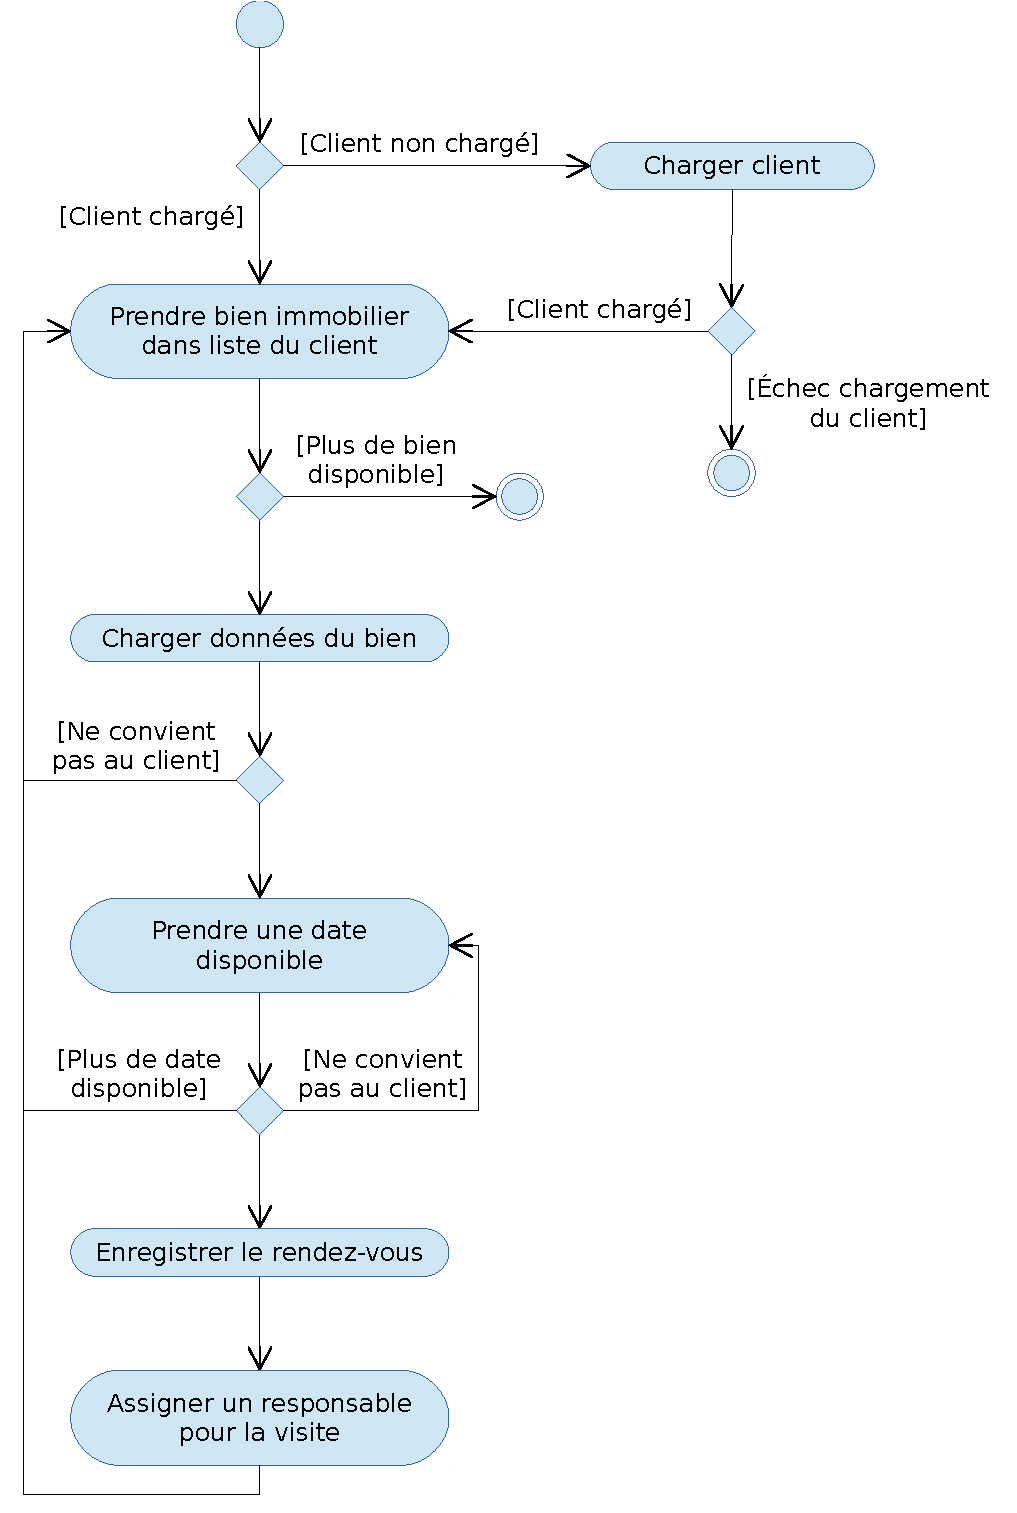
\includegraphics[scale=0.67]{IMG/ad}
  \caption{Diagramme d'activitéss}
  \label{img_ad}
\end{figure}

La figure \refpage{img_ad} illustre le diagramme d'activité du cas d'utilisation \og{}Visiter un bien\fg{}.

\section{Rapport}

%J'ai réalisé ce diagramme en troisième lieu. Il est basé sur le diagramme entités-associations et représente la structure des différentes données qui seront implémentées. Nous nous sommes ici plus proche de la réalité que du conceptuel.

%Les entités ont été remplacées par des classes. Les associations ont été remplacées soit par des attributs, soit par des classes suivant les cas.